We will now review with the kernel implementation.

\subsection{Kernel writing}
The kernel in itself is written in CUDA in the GASAL2 library. It should exactly replicate the behaviour of the original function in BWA, called \verb|ksw_extend|. From there on, we will refer to the original function with this name, and to its GPU implementation as the \verb|ksw_kernel|.

We have seen before that previous kernels in GASAL2 were written as C++ template functions. It has been considered using the already existing local alignment kernel template to derive an alternate kernel with the starting scores. This could have reduced the amount of code to maintain. However, the more we investigated this possibility, the more differences we found out between the to-be seed-only kernel and the local kernel we had. In particular, an important number of speed-up techniques were present in \verb|ksw_extend| and marked a high level of difference with the previous solution. For the sake of simplicity, we created a new kernel dedicated to the seed-only paradigm.

The kernel has been built by copying the original \verb|ksw_extend| and renaming the variables to plug it into the naming convention used in GASAL2 kernels. At first, we followed the loop structure used in \verb|ksw_extend| in which there is no data compression. The behaviour is simply to fetch the current base from query and the current base from target and calculate the cell of the dynamic programming matrix. Therefore, the pseudocode is the same as presented previously in Algorithm~\ref{algo:local}.

Secondly, we introduced the use of compressed data by fetching the 8 bases in the 32-bit words from query and target. This added two innermost loops in the algorithm to perform the alignment tile by tile, using square tiles of $8 \times 8 = 64$ bases.

Because of memory constraints, the whole matrix is not stored in memory. Instead, only a full row having the length of the query string is stored. For the record, only the north, west, and north-west cells are needed for the computation. This is shown on Figure~\ref{fig:visualisation-aid-tile}. All cells are computed in the order given by their number. When a full column is computed, the orange column moves one step on the right, taking the place of the cells numbered 1 to 8, then cells 9 to 16 when they are computed, and so on. This column is the western cells used to compute the score. When all cells in the tile are computed, the 8-cell section of the yellow row moves 8 cells down, taking the place of the cells numbered 8, 16, 24 ... 64. When the cyan tile is computed, it goes to the blue one, then the navy blue, then the next line.

\begin{figure}[h!]
	\centering
	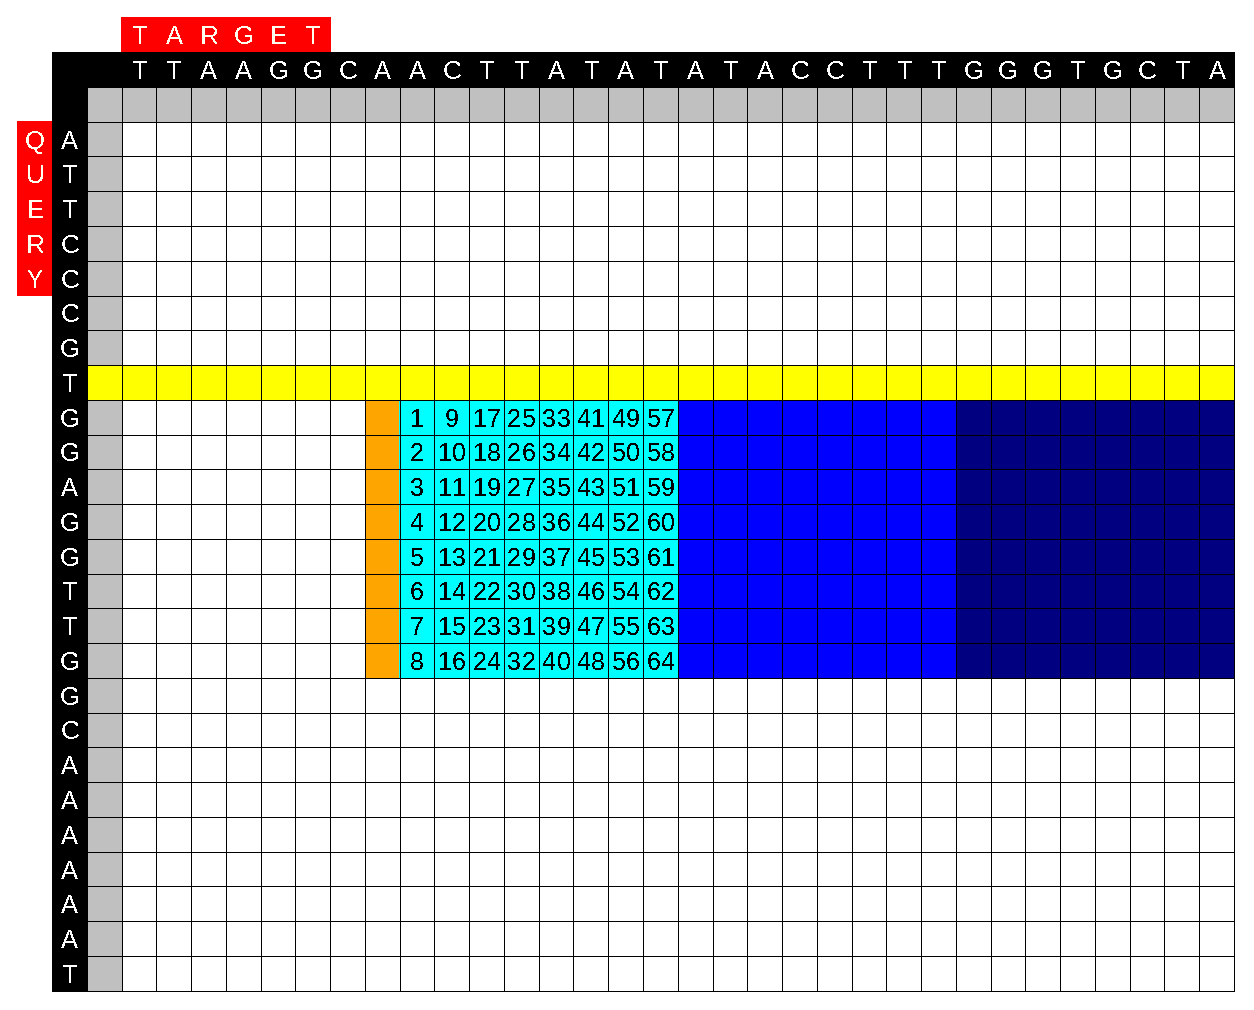
\includegraphics[width=0.9\linewidth]{visualisation-aid-tile}
	\caption{Visualisation of the tile-based matrix computation. Only the yellow row and the orange column are stored in memory.}
	\label{fig:visualisation-aid-tile}
\end{figure}

%The algorithm changes as reported in paper ~\cite{Ahmed:gasal}.

Finally, we introduced again some computing optimisation that we disabled in the second version of the kernel, in particular, z-dropoff. This optimisation allows to skip the calculation of some cells of the matrix provided the score drops below a certain threshold. When this happens, it usually means that the alignment will not improve because the difference between the two sequences grew too big, so it is usually better to stop computing altogether instead of wasting time trying to align two sequences that are visibly very different.

\subsection{Score comparison}

To verify the correctness of this implementation, a modified version of BWA is made from the original BWA~\cite{lh3:bwa}. This version is hosted on GitHub~\cite{j-levy:bwa} and has different branches to switch from one behaviour to another, to compare the results with the GPU-accelerated implementation.

In a branch called \verb|no-zdrop-seedonly|, we introduced our seed-only method instead of the original BLAST-like behaviour. As the name suggests, we also disabled the z-dropoff when comparing the result for this branch, but we re-introduced it afterwards to check the implementation of the z-dropoff in GASAL2, and verified that they matched.

The results are in the Sequence Alignment/Map (SAM) format, commonly used for DNA alignment. SAM is text-based, extensively documented~\cite{samtools:sam} and widespread among DNA-related programs. It is the default format output for BWA. Using \verb|diff| and other regular UNIX tools, we can compare the number of lines that differ between the reference program and a modified version. Knowing the original number of lines, we can derive a percentage of difference between the files, as shown on Listing~\ref{lst:diff}.

\begin{listing}[ht]
	\begin{minted}[
	fontsize=\footnotesize,
	linenos,
	breaklines,
	frame=single]{bash}
#!/bin/bash
DIFFLINES=$(diff --suppress-common-lines --speed-large-files -y $1 $2 | grep "[|><]" | wc -l)
TOTALLINES1=$(cat $1 | wc -l)
PERCENTDIFF=$(bc -l <<< "scale=2; (100*$DIFFLINES)/$TOTALLINES1")

echo "Different lines between " $1 " and " $2 " = " $DIFFLINES
echo "Total numer of lines in" $1 " = " $TOTALLINES1
echo "Difference = " $PERCENTDIFF "%"
	\end{minted}
	\caption{Bash script to show percentage of difference between two files}
	\label{lst:diff}
\end{listing}

